\appendix

\section{Process Flow}

\begin{table}[H]
\centering
\scriptsize
\setlength{\tabcolsep}{2.5pt}
\renewcommand{\arraystretch}{0.95}
\begin{tabularx}{\textwidth}{l l l X}
\toprule
\textbf{Process Activity} & \textbf{Resource} & \textbf{Patient type} & \textbf{Data} \\
\midrule

\multicolumn{4}{l}{\textbf{Administrative}} \\
Sign in & Front desk & All & New: 30, Other: 15 min \\
Register & Front desk & All & Avg: 4.33 min \\
Check-Out & Front desk & All & Avg: 4.72 min \\

\midrule
\multicolumn{4}{l}{\textbf{Clinical}} \\
Vitals & CA, Exam room & All & Avg: 3.53 min \\
Resident review & Resident & New/Return & New: 10.44, Return: 9.30 min \\
Resident \& Patient & Resident, Exam room & New/Return & New: 20.16, Return: 12.99 min \\
Teach & Resident, Attending & New/Return & New: 7.85, Return: 5.17 min \\
Resident \& Attending & Resident, Attending, Exam room & New/Return & New: 12.45, Return: 9.24 min \\

\midrule
\multicolumn{4}{l}{\textbf{Follow-up}} \\
PA consultation & PA, exam room & Follow-up & -- \\
PA \& Attending & PA, Attending & Follow-up (50\%) & Approx. 3 min \\

\bottomrule
\end{tabularx}
\caption{Process activities}
\label{tab:process}
\end{table}

\section{Flow chart}
\setcounter{figure}{0}

\begin{figure}[H]
    \centering
    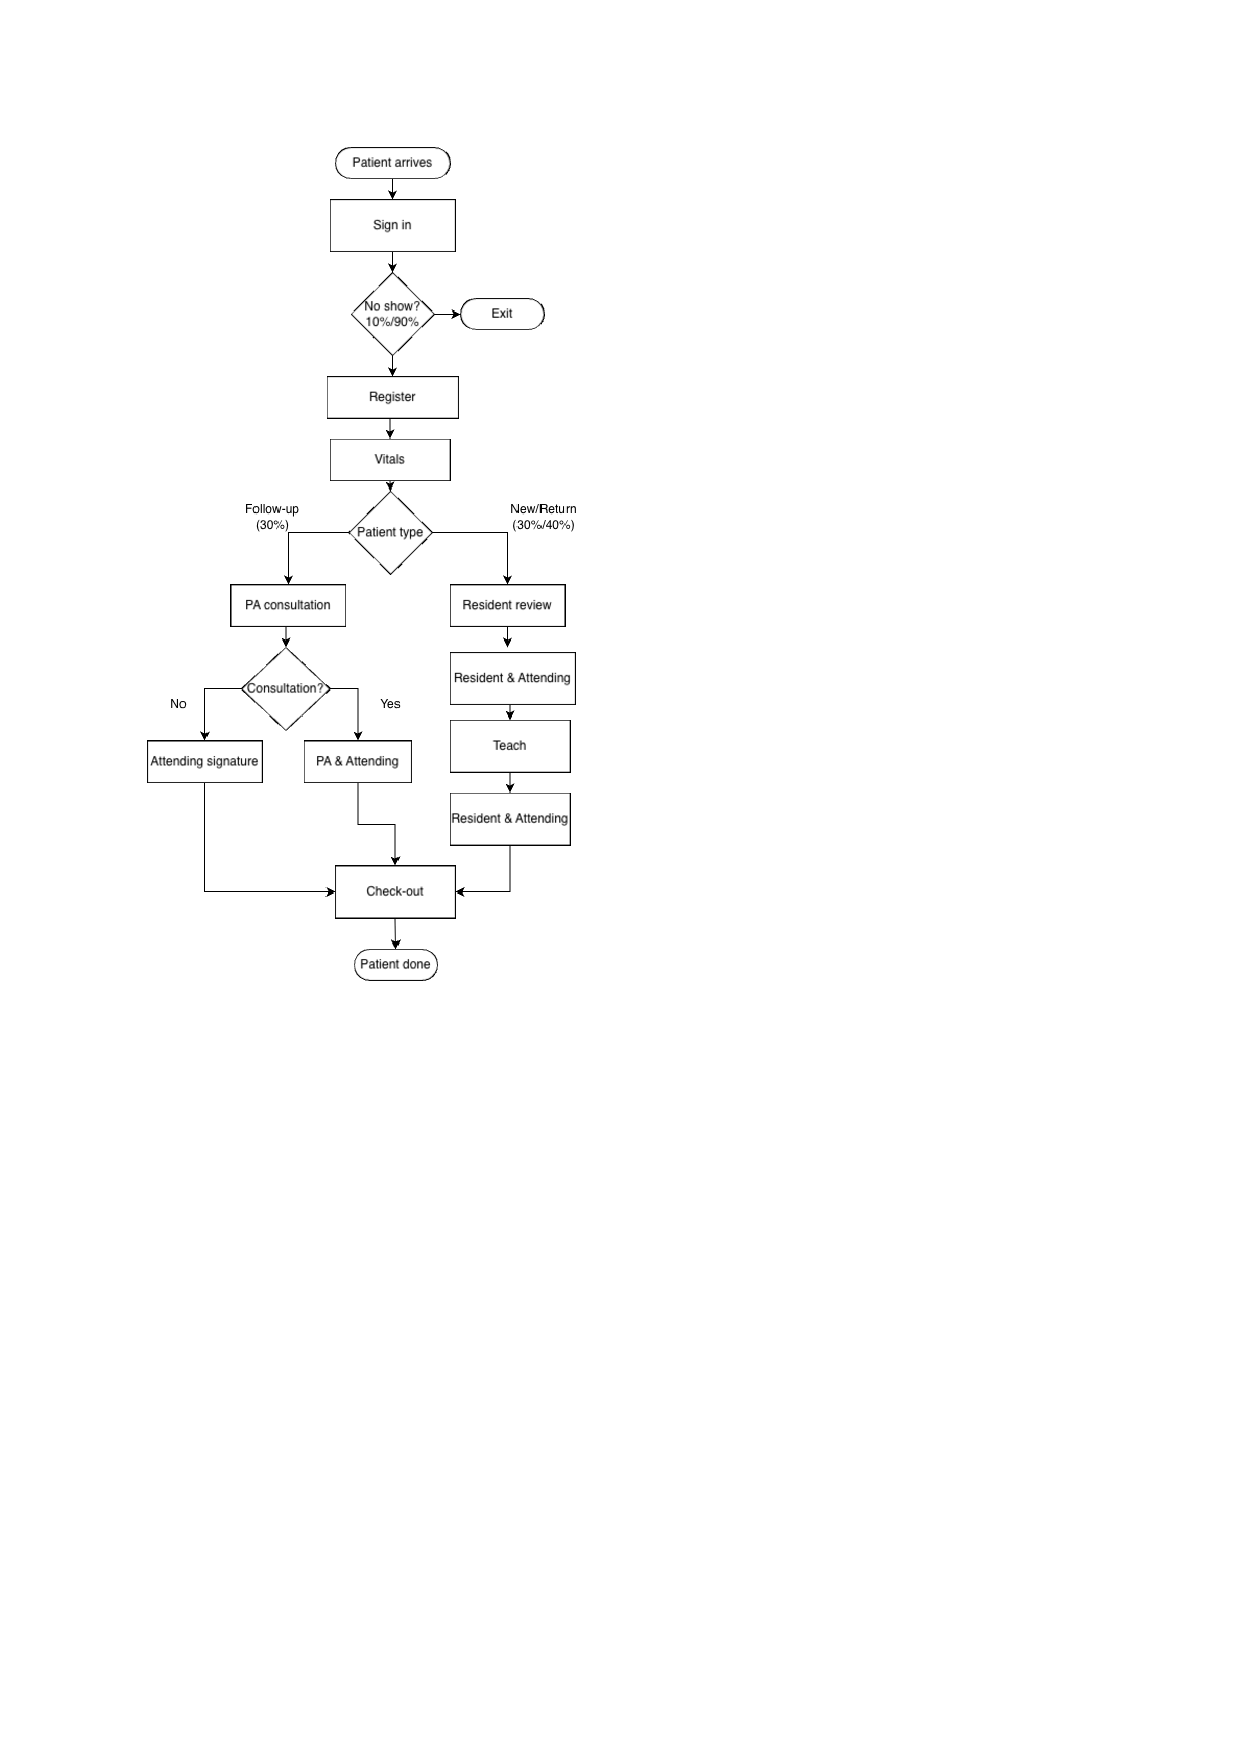
\includegraphics[width=0.7\textwidth]{Inputs/Pictures/FlowChart.pdf}
    \caption{Flow chart}
    \label{fig:FlowChart}
\end{figure}

\section{Conceptual design}
\setcounter{table}{0}

\begin{table}[H]
\centering
\scriptsize
\setlength{\tabcolsep}{3pt}
\renewcommand{\arraystretch}{0.9}
\begin{tabularx}{\textwidth}{
>{\raggedright\arraybackslash}p{0.22\textwidth}
>{\raggedright\arraybackslash}p{0.20\textwidth}
>{\raggedright\arraybackslash}X}
\toprule
\textbf{Components} & \textbf{Simulation implementations} & \textbf{Specifications \& resources} \\
\midrule

\multicolumn{3}{l}{\textbf{Arrival and routing}} \\
Patient & SimEntity & One entity type. Patient type decided by PatientType Branch \\
Scheduled arrivals & EntityGenerator, EventSchedule & 17 patients per schedule; max=17; cycle=10 h \\
No-show decision & Branch & P(continue)=0.90 $\rightarrow$ Registration; P(no-show)=0.10 $\rightarrow$ exit; sign in instantaneous \\
Patient type routing & Branch & P(new)=0.30, P(return)=0.40, P(follow-up)=0.30 \\
PA consultation? & Branch & P(consult)=0.50, P(not)=0.50 \\

\midrule
\multicolumn{3}{l}{\textbf{Common input flow}} \\
Register & Server, Queue & Gamma(mean=4.333 min, shape=3.069) \\
Vitals & Server, Queue & Weibull(scale=3.982 min, shape=2.107) \\

\midrule
\multicolumn{3}{l}{\textbf{New and return flow}} \\
Resident Review & Seize, Server, Queue & Seize resident \& exam room. New: Gamma(mean=10.4). Return: LogNormal($\mu$=1.737, $\sigma$=1.002) \\
Resident \& Patient & Server, Queue & New: LogNormal($\mu$=2.857, $\sigma$=0.558), Return: Weibull(scale=14.665, shape=1.740) $\rightarrow$ SeizeAttending \\
Teach & Seize, Server, Queue & SeizeAttendingResource. New: Gamma(mean=7.861), Return: Weibull(scale=5.438) \\
Resident \& Attending & Server, Queue & New: Gamma(mean=12.450), Return: LogNormal($\mu$=1.942, $\sigma$=0.738); release all $\rightarrow$ check-out \\

\midrule
\multicolumn{3}{l}{\textbf{Follow-up flow}} \\
PA & Seize, Server, Queue & Seize PA room. LogNormal($\mu$=2.968, $\sigma$=0.541) \\
PA \& Attending & Seize, Server, Queue & Seize Attending; constant=3 min; release $\rightarrow$ check-out \\

\midrule
\multicolumn{3}{l}{\textbf{Departure flow and output}} \\
Check-Out & Server, Queue & Gamma(mean=4.724, shape=2.320) $\rightarrow$ PatientStatistics $\rightarrow$ Exit \\
Output & Statistics, EntitySink & PatientStatistics collect total time per patient \\

\midrule
\multicolumn{3}{l}{\textbf{Resources}} \\
Attending & Resource & Capacity=1 (New, Return, Follow-up) \\
Residents & Resource & Capacity=3; held from Resident Review to Resident \& Attending \\
Exam room (New/Return) & Resource & Capacity=3; held from Resident Review to Resident \& Attending \\
PA exam room & Resource & Capacity=1; dedicated Follow-up; held from PA to PA \& Attending \\

\bottomrule
\end{tabularx}
\caption{Simulation components, implementations, specifiations and resources}
\label{tab:conceptual_design}
\end{table}

\section{Stochastic variables}

\begin{table}[H]
\centering
\small
\begin{tabularx}{\textwidth}{p{4cm} p{2cm} X}
\toprule
\textbf{Variable} & \textbf{Type} & \textbf{Description} \\
\midrule

\multicolumn{3}{l}{\textbf{Service times}} \\
Registration time & Continuous & Time spent on administrative registration \\
Vitals time & Continuous & Time to record patient vitals \\
Physician assistant time & Continuous & Time spent by PA on follow-up patients \\
Check-out time & Continuous & Time to complete visit and paperwork \\
Resident review (new) & Continuous & Time reviewing patient file (new patients) \\
Resident--patient interaction (new) & Continuous & Consultation time with resident \\
Teaching time (new) & Continuous & Teaching interaction between resident and attending \\
Resident--attending interaction (new) & Continuous & Discussion between resident and attending \\
Resident review (return) & Continuous & Time reviewing file (return patients) \\
Resident--patient interaction (return) & Continuous & Consultation time with resident \\
Teaching time (return) & Continuous & Teaching interaction for return patients \\
Resident--attending interaction (return) & Continuous & Discussion between resident and attending \\

\midrule
\multicolumn{3}{l}{\textbf{Routing decisions}} \\
Patient type & Discrete & New, return, or follow-up patients \\
Follow-up requires attending & Discrete & Whether PA consults attending (approximately 50\%) \\
No-show / cancellation & Discrete & Whether patient attends appointment (approximately 10\% no-show) \\

\bottomrule
\end{tabularx}
\caption{Identified stochastic inputs}
\label{tab:stochastic_vars}
\end{table}

\newpage
\section{JaamSim documentation}

\section{AS-IS}

The AS-IS model simulates the Miller Pain Treatment Center in its current state. Patients arrives at their scheduled appointments, with 17 appointments between 08:00 and 11:15. A 10\% no-show rate is applied with a branch at arrival, from the case description.

After registration and vitals, patients are routed by type. New and return patients seize a resident and an examination room before going through resident processes with attending and teaching. Follow-up patients seize a examination room and are seen by a physical assistant, with a 50\% probability of needing additional medical attention. 

Service time distributions were fitted from the data provided in the case given in \cite{MillerPainTreatmentCenter}, with the distributions given in \autoref{tab:finalinputs}.

\section{TO-BE 1: Scheduling}

The TO-BE 1 (Scheduling) is identical to the AS-IS model in its structure. The only modification done is changing of the patient schedule, where all appointments are evenly spread every 15 minutes throughout each session. This is done after Dr. Weems suspicion that clustered appointments contribute to inefficiency in the system \parencite{MillerPainTreatmentCenter}.

\section{TO-BE 2: Pre-processing}

Dr. Weems also suspects that the variance accross teaching contributes to performance loss in the system, suggesting that reviewing the case the day before might decrease waiting times in this area. Dr. Weems estimates that this could cut average review- and teaching times in half \parencite{MillerPainTreatmentCenter}. We have therefore halved distributions connected to these processes, while all other variables are kept intact.

\section{TO-BE 1: Combined}

The combined model simulates a system where both scheduling and pre-processing are used, to see if a combination of the two modifications provide better performance than either alone. This model builds on the thought that Dr. Weems assumptions about scheduling and pre-processing are independent performance factors, and that applying both simultaneously might provide better results.